\documentclass[a4paper,10pt,twocolumn]{ltjsarticle}
\usepackage[haranoaji]{luatexja-preset}
\usepackage[top=16mm,bottom=18mm,left=15mm,right=15mm,columnsep=6mm]{geometry}
\usepackage{amsmath,amssymb,mathtools}
\usepackage{booktabs,tabularx,array,multirow}
\usepackage{siunitx}
\usepackage{xcolor}
\usepackage{tikz}
\usetikzlibrary{arrows.meta,positioning,fit,calc}
\usepackage[hidelinks]{hyperref}
\usepackage{enumitem}
\usepackage{listings}
\usepackage{caption}
\captionsetup{font=small,labelfont=bf}
\setlength{\parindent}{1em}
\setlength{\parskip}{0pt}
\setlist{nosep,leftmargin=1.8em}
\newcommand{\code}[1]{\texttt{#1}}
\newcommand{\R}{\mathrm{R}}
\newcommand{\Lsym}{\mathrm{L}}
\newcommand{\Nsym}{\mathrm{N}}
\newcommand{\high}{\mathrm{HIGH}}
\newcommand{\low}{\mathrm{LOW}}
\newcommand{\main}{\mathrm{main}}
\newcommand{\block}{\mathrm{blocked}}
\newcommand{\rank}{\operatorname{rank}}
\newcommand{\unrank}{\operatorname{unrank}}
\title{\textbf{GPUフロンティアDPにおけるMotzkin状態空間の因数分解と\\ZDD復元時の変数順序最適化}\\[-1mm]
\large 正方格子の対角頂点間自己回避路の厳密数え上げに向けた予備評価}
\author{GPT-5.6 Sol\thanks{本稿はGPT-5.6 Solが研究実装、実験設計、実験実行および原稿作成を行った予備稿である。所属なし。}}
\date{2026年8月22日 -- v0.3 preliminary manuscript}

\begin{document}
\maketitle

\begin{abstract}
正方格子の対角頂点間を結ぶ自己回避路の厳密数え上げは、状態数が格子幅に対して指数的に増加する代表的なフロンティア動的計画法（frontier DP）の応用である。本研究では、最小完全ハッシュに基づく既存のMotzkin型状態符号化をGPU向けに再構成し、状態を固定分割境界の中間高さで因数分解する\emph{factorized topology codec}を提案する。従来GPU実装では、各行・各CRT法の剰余計算で同一のトポロジに対してrank/unrankを繰り返していた。提案法は、状態集合を中間高さごとの直積 $\high_h\times\low_h$ の非交和として表し、半幅の符号表と小規模なprefix表のみを保持することで、遷移先rankとcanonical rankの大部分を表引きと加減算に置き換える。

NVIDIA GeForce RTX 3070上の単一剰余計算では、セル幅 $n=18,20,21$ に対して、それぞれ15.96\%, 28.16\%, 25.83\%の実行時間短縮を確認した。$n=21$ では69.53秒から51.57秒へ短縮し、遷移部だけでは53.56秒から36.82秒へ31.26\%短縮した。複数の法に対する剰余値および既存実装との一致を確認している。さらに、Grid-FPの遷移をreplayして全実辺を変数とするZDDを復元し、変数順序を広域siftingで最適化した。$n=6$--10では、一般化した\emph{wave2}順序により標準row-major順と比べ18.87--25.52\%のZDDノード削減を得た。次の未掲載項を狙うセル幅 $n=27$（頂点幅28）では、factorized codec表の追加メモリは既存LOW表を共用した場合に約286 MiB/GPUと見積もられ、8基のB300級GPUで現実的な範囲に収まる。本稿では、GPU上の状態トポロジ計算と、計算後の解集合をZDDとして復元・保存する際の変数順序の双方を報告する。
\end{abstract}

\noindent\textbf{キーワード:} フロンティアDP, 自己回避路, GPU, CUDA, Motzkin path, 最小完全ハッシュ, CRT, ZDD, 変数順序

\section{はじめに}
正方格子上で一方の隅から対角の隅まで、頂点を二度訪れずに進む路の本数を求める問題は、OEIS A007764として長く研究されてきた\cite{oeis}。閉形式は知られておらず、厳密値の更新はアルゴリズムと計算機資源の両方に強く依存する。KnuthのSIMPATH/ZDD系の考え方\cite{knuth4a}を基礎として、IwashitaらはZDDによる列挙\cite{iwashita2012}、さらに格子専用の状態圧縮と最小完全ハッシュによる動的計画法\cite{iwashita2013}を開発した。現在OEISには頂点幅27までの値が掲載されている\cite{oeis}。

本稿では表記をGPU実装に合わせ、\textbf{$n\times n$セル、$(n+1)\times(n+1)$頂点}の格子を問題サイズ$n$とする。したがって本稿で目標とする$n=27$は頂点幅28であり、OEIS A007764の次の未掲載項に対応する。この表記差は既存文献との比較時に特に重要である。

既存CPU法の主要な工夫は、フロンティア上の連結性を非交差括弧列として表現し、Motzkin pathに対応する状態をrank/unrankで密な整数区間へ写像することである。GPU化では密配列が有利である一方、巨大状態空間をVRAMに収めるために状態をoccupancy maskでgroup化し、局所windowだけをscratchへ取り出して更新する必要がある。本研究で用いたベースラインは、2つの固定window、LOW/HIGH LUT、rank差分、blocked状態のdrop-$N$ rank、複数GPU間のHBM shardingを組み合わせたCUDA実装である。

本研究の主な貢献は次の5点である。
\begin{enumerate}
  \item Motzkin状態を中間高さで厳密に直積分解し、group local rank/unrankとcanonical rankを半幅表から再構成する\emph{factorized topology codec}を導入した。
  \item RTX 3070上で$n=18,20,21$を評価し、最大28.16\%、$n=21$で25.83\%の総実行時間短縮を得た。遷移部単体では31.26\%短縮した。
  \item 対称性MITM、最初の1辺固定、per-state topology cache、単純なrank再利用など複数の代替案を実験し、スケールしない理由を定量化した。
  \item Grid-FPの状態遷移を再実行して全実辺を変数とするZDDを復元するreplay exporterを実装し、独立SIMPATH型builderとの集合族一致およびSAPPOROBDD互換出力を確認した。
  \item ZDD復元時の変数順序を実験的に最適化し、最大frontier幅を増やさない\emph{wave2}順序により、標準row-major順に対して$n=6$--10で18.9--25.5\%のZDDノード削減を得た。
\end{enumerate}

\section{問題設定と既存フロンティアDP}
\subsection{フロンティア状態}
セルを一定順序で走査し、既処理領域と未処理領域の境界（frontier）に現れる部分路の接続関係を状態として保持する。平面格子では接続が交差しないため、各frontier位置は
\[
\Nsym\;(未使用),\qquad \R\;(右括弧),\qquad \Lsym\;(左括弧)
\]
の3値で表せる。外部端点に対応するdefectを1つ含むため、状態列は初期高さ1のMotzkin pathとみなせる。高位位置から低位位置へ走査するとき、$\R$で高さを1下げ、$\Lsym$で1上げ、$\Nsym$で不変とし、最終高さ0となる列のみが合法状態である。

幅$W=n+1$に対するmain状態数を$M(W)$とする。本実装で観測される代表値は
\[
M(22)=728{,}997{,}192,\qquad
M(28)=385{,}719{,}506{,}620
\]
である。blocked状態は幅が1小さく、$W=28$では135,015,505,407状態となる。通常のMotzkin数を$\mathrm{Motzkin}_k$とすると、本実装のmain状態数は
\[
M(W)=\mathrm{Motzkin}_{W+1}-\mathrm{Motzkin}_{W}
\]
と書ける。各状態を32 bit剰余1個で保持した場合、$n=27$のauthoritative stateは約1939.89 GiB、すなわち約1.894 TiBに達する。

\subsection{rank/unrankとGPU上の問題}
Iwashitaらの最小完全ハッシュは、合法Motzkin状態だけを$[0,M(W))$へ密に対応させる\cite{iwashita2013}。GPUではこの密配列によりハッシュテーブルを避けられるが、group化した部分状態を処理する際に次の処理が頻繁に現れる。
\begin{itemize}
  \item group local indexからMateIDを復元する$\unrank$;
  \item 遷移後MateIDのgroup local $\rank$;
  \item canonical authoritative配列のglobal $\rank$;
  \item main状態からblocked状態へ1位置を落とすrank変換。
\end{itemize}
これらは\textbf{modulusにもrowにも依存しない}にもかかわらず、従来実装では各row、さらにCRTの各剰余ごとに再計算されていた。

\subsection{固定2-window GPU実装}
$n=27$向けベースラインはfrontierを2つのwindowに分ける。$W=28$では概念的に
\[
\underbrace{\high_{13}}_{13\text{位置}}\;\;c\;\;
\underbrace{\low_{14}}_{14\text{位置}}
\]
とし、上側windowと下側windowを交互に処理する。各windowの外側ではoccupancyを固定して独立なgroupを形成する。状態値は全GPUのHBMへshardし、groupをscratchへgatherし、複数の局所辺更新を行い、scatterでauthoritative配列へ戻す。

\begin{figure}[t]
\centering
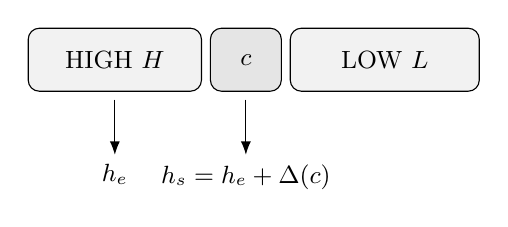
\begin{tikzpicture}[font=\small,>=Latex]
  \node[draw,rounded corners,minimum width=22mm,minimum height=8mm,fill=gray!10] (h) {HIGH $H$};
  \node[draw,rounded corners,minimum width=9mm,minimum height=8mm,fill=gray!20,right=1mm of h] (c) {$c$};
  \node[draw,rounded corners,minimum width=24mm,minimum height=8mm,fill=gray!10,right=1mm of c] (l) {LOW $L$};
  \draw[-{Latex}] ($(h.south)+(0,-1mm)$) -- ++(0,-7mm) node[below] {$h_e$};
  \draw[-{Latex}] ($(c.south)+(0,-1mm)$) -- ++(0,-7mm) node[below] {$h_s=h_e+\Delta(c)$};
\end{tikzpicture}
\caption{main状態の分割。HIGHを通過した中間高さ$h_e$とcenter記号$c$によりLOW開始高さ$h_s$が決まる。}
\label{fig:split}
\end{figure}

\section{提案法: Factorized Topology Codec}
\subsection{状態集合の直積分解}
main状態の幅を
\[
W=H+1+L
\]
とする。HIGH部分を初期高さ1から終端高さ$h_e$へ到達する合法列の集合$\high_{h_e}$、LOW部分を開始高さ$h_s$から0へ到達する合法列の集合$\low_{h_s}$とする。center記号$c\in\{\Nsym,\R,\Lsym\}$の高さ変化を
\[
\Delta(\Nsym)=0,\quad \Delta(\R)=-1,\quad \Delta(\Lsym)=+1
\]
とすれば、main状態集合$\mathcal{S}_{\main}$は
\begin{equation}
\mathcal{S}_{\main}
=\biguplus_{h_e}\;\biguplus_{c}
\left(\high_{h_e}\times\{c\}\times\low_{h_e+\Delta(c)}\right)
\label{eq:factor-main}
\end{equation}
と分解できる。不正な高さの場合は対応集合を空とする。一方blocked状態にはcenterがないため
\begin{equation}
\mathcal{S}_{\block}
=\biguplus_h \left(\high_h\times\low_h\right).
\label{eq:factor-block}
\end{equation}
これは近似ではなく、Motzkin高さの連続性から直接得られる完全な非交和である。

各ブロック内でHIGH rankを$r_H$、LOW rankを$r_L$、LOW状態数を$s_L$とすると、group local indexは
\begin{equation}
 i=\mathrm{offset}(h,c)+r_H s_L+r_L
\label{eq:localrank}
\end{equation}
で与えられる。逆写像は整数除算と剰余、および半幅code table参照だけで得られる。

\subsection{occupancy maskとの整合}
固定2-windowでは一方の半分のoccupancy maskが固定される。提案法では各半幅codeについて
\begin{itemize}
  \item 全合法codeを高さ別に並べた\code{all\_codes};
  \item occupancy maskと高さ別に並べた\code{mask\_codes};
  \item 2bit/位置で表したcodeからall rankとmask rankを同時に取得する\code{packed\_rank};
\end{itemize}
を構築する。window A/Bで固定側が入れ替わっても、式\eqref{eq:localrank}のHIGH/LOW rank参照先を切り替えるだけでよい。

これにより、従来の「幅$W$のMotzkin DP表を高位から低位まで走査してrank/unrank」を、半幅table lookupと小数回の算術へ置換できる。

\subsection{canonical global rankの$O(1)$化}
局所groupだけでなくauthoritative canonical配列のglobal rankも同じ分解で計算できる。本稿では、全状態値をcanonical rank順に保持する正規配列を\emph{authoritative array}と呼ぶ。記号順序を$\Nsym<\R<\Lsym$とする。

main状態ではHIGH codeに依存するprefix寄与を$B_H^{\main}$、center記号より前の合法分岐の寄与を$B_c^{\main}$とし、LOW codeのall rankを$r_L^{\mathrm{all}}$とすると、
\begin{equation}
\rank_{\main}(H,c,L)
=B_H^{\main}(H)+B_c^{\main}(h_e,c)
+r_L^{\mathrm{all}}(L;h_e+\Delta(c)).
\label{eq:globalrank-main}
\end{equation}
ここで
\begin{equation}
B_c^{\main}(h,c)
=\sum_{c'<c,\;h+\Delta(c')\ge0}
|\low_{h+\Delta(c')}|
\end{equation}
である。一方blocked状態では残りsuffix長がmainとは異なるため、main用prefixからcenter項を単純に除くのではなく、blocked専用のprefix $B_H^{\block}$を用いて
\begin{equation}
\rank_{\block}(H,L)
=B_H^{\block}(H)+r_L^{\mathrm{all}}(L;h)
\label{eq:globalrank-block}
\end{equation}
とする。これにより両rankを半幅table lookupと加算のみで求められる。

実装初期版ではhost側prefix表生成で、定数$L$が列挙値$\Lsym$をshadowするバグが生じた。幅4--12の全状態照合とGPU上のgather時比較により原因を特定し、修正後は既存global rankと一致した。この検証は、式そのものと表生成実装を分離して確認する上で有用であった。

\begin{figure}[t]
\centering
\begin{tikzpicture}[font=\footnotesize,>=Latex,node distance=4mm]
\node[draw,rounded corners,align=center] (old1) {local index};
\node[draw,rounded corners,align=center,right=of old1] (old2) {full-width\\unrank};
\node[draw,rounded corners,align=center,right=of old2] (old3) {MateID};
\node[draw,rounded corners,align=center,right=of old3] (old4) {full/partial\\rank};
\draw[->] (old1)--(old2);\draw[->](old2)--(old3);\draw[->](old3)--(old4);
\node[below=9mm of old2,align=center] (lab) {提案法};
\node[draw,rounded corners,align=center,left=3mm of lab] (new1) {local index};
\node[draw,rounded corners,align=center,right=3mm of lab] (new2) {half tables\\+ offset};
\node[draw,rounded corners,align=center,right=of new2] (new3) {target rank};
\draw[->](new1)--(new2);\draw[->](new2)--(new3);
\end{tikzpicture}
\caption{従来と提案codecの概念比較。提案法はrow/modulus非依存のトポロジを半幅表へ移す。}
\label{fig:codec}
\end{figure}

\subsection{メモリ量}
$n=27$向けの$L=14,H=13$では、生成されたvalid code数はLOW 1,201,917、HIGH 787,333であった。dense packed-rank表はLOWが1024 MiB、HIGHが256 MiBである。LOW dense tableは既存LOW LUTのdense rank領域と役割を統合可能であり、二重保持する必要はない。その他のcode配列、offset、HIGH prefix baseを合計すると、\textbf{既存LOW表を共用した純増は約286 MiB/GPU}と見積もられる。

B300 $\times8$を想定した$n=27$ authoritative stateはmain 385,719,506,620状態、blocked 135,015,505,407状態で、32bit剰余では計約1939.89 GiB、8分割時約242.49 GiB/GPUである。したがって286 MiBはauthoritative stateに比べて0.12\%程度であり、十分小さい。

\section{正当性}
\paragraph{補題1（直積分解）}
合法なmain Motzkin状態$m$をHIGH、center、LOWへ切ると、HIGH終了高さ$h_e$とcenter$c$は一意であり、LOW開始高さは$h_e+\Delta(c)$で一意に定まる。逆に、式\eqref{eq:factor-main}の任意の組を連結すると初期高さ1、非負、終端高さ0の合法状態となる。よって式\eqref{eq:factor-main}は全単射である。blockedも同様に式\eqref{eq:factor-block}が成り立つ。

\paragraph{補題2（局所rank）}
各$(h,c)$ブロック内でHIGHを外側、LOWを内側に辞書順列挙すれば、式\eqref{eq:localrank}は通常の直積集合のrow-major rankであり全単射である。occupancy maskで片側を制限した場合も、その集合を\code{mask\_codes}へ置換するだけで同じ議論が成り立つ。

\paragraph{補題3（canonical rank）}
最小完全ハッシュのrankは、高位から順に現在記号より小さい合法分岐のsuffix数を加算する。HIGH部分に起因する和はHIGH codeだけで決まり前計算可能である。centerの寄与は$h_e,c$だけで決まり、残るLOW部分は開始高さ固定のall rankである。したがって式\eqref{eq:globalrank-main}および式\eqref{eq:globalrank-block}は従来rankと一致する。

以上より、factorized codecは状態集合・局所rank・canonical rankを変更せず、表現と計算順序だけを変える。DPの算術遷移が同一である限り、各modulusに対する最終剰余も同一となる。

\section{実験}
\subsection{環境}
開発機の構成を表\ref{tab:env}に示す。GPU性能表の計測はshard数1の単一GPU、32bit modulus、同一の固定2-window構成で行った。時間はsolverが報告するrow-loop本体のwall-clockであり、table構築、allocation、初期zeroing、ファイルI/Oは含めない。各値はwarm-up後の代表1実行であり平均値ではない。$n=18$では複数modulusによる回帰も行った。

\begin{table}[t]
\centering
\caption{開発・評価環境}
\label{tab:env}
\begin{tabular}{ll}
\toprule
GPU & GeForce RTX 3070, 8 GiB\\
CPU & Intel Core i7-12700\\
CUDA & 13.3 (nvcc 13.3.73)\\
Driver & 610.57.04\\
OS & Linux 7.1.8-1-cachyos x86\_64\\
Compiler option & \code{-O3 -std=c++17}\\
\bottomrule
\end{tabular}
\end{table}

\subsection{総実行時間}
表\ref{tab:perf}に結果を示す。$n=18$では15.96\%、$n=20$では28.16\%、$n=21$では25.83\%短縮した。$n$が大きくなるにつれrank/unrankが占める割合が増えるため、$n=20,21$で効果が大きい。

\begin{table*}[t]
\centering
\caption{RTX 3070における単一剰余の実行時間。Baselineは固定2-window + LOW/HIGH LUT + rank差分を用いる実装。}
\label{tab:perf}
\begin{tabular}{rrrrrr}
\toprule
$n$ & modulus & Baseline [s] & Factorized [s] & speedup & 時間短縮\\
\midrule
18 & 4294967291 & 4.49608 & 3.77839 & 1.190$\times$ & 15.96\%\\
20 & 4294967291 & 25.7445 & 18.4950 & 1.392$\times$ & 28.16\%\\
21 & 4294967291 & 69.5275 & 51.5680 & 1.348$\times$ & 25.83\%\\
\bottomrule
\end{tabular}
\end{table*}

\subsection{正しさの回帰}
$n=18$で3種類のmodulusを連続実行し、既存forced2実装と同一の剰余を得た。
\begin{center}
\begin{tabular}{rr}
\toprule
modulus & residue\\
\midrule
4294967291 & 503411004\\
4294967279 & 2737033518\\
2147483647 & 624312750\\
\bottomrule
\end{tabular}
\end{center}
さらに$n=20$では2308006916、$n=21$では998035516が双方の実装で一致した。これらは実装上のfactor table、局所rank、global rank、およびmain/blocked遷移が整合していることを確認する回帰試験として用いた。

\subsection{プロファイル}
$n=21$についてgather、transition、scatterへ分けた結果を表\ref{tab:profile}に示す。提案法の主効果はtransitionに現れ、53.56秒から36.82秒へ31.26\%短縮した。gatherは8.54秒から8.78秒へわずかに悪化し、scatterは7.41秒から6.07秒へ短縮した。総時間はprofile build同士で25.65\%短縮した。

\begin{table}[t]
\centering
\caption{$n=21$の処理内訳 [s]}
\label{tab:profile}
\begin{tabular}{lrr}
\toprule
区間 & Baseline & Factorized\\
\midrule
gather & 8.54 & 8.78\\
transition & 53.56 & 36.82\\
scatter & 7.41 & 6.07\\
\midrule
合計 & 69.52 & 51.68\\
\bottomrule
\end{tabular}
\end{table}

この結果は、「HBM帯域だけを改善した」のではなく、transition中で繰り返されていたトポロジrank計算を除去したことが主要因であることを示す。一方gather/scatterには依然約14.85秒が残り、今後の直接repartitionやfactorized authoritative layoutの余地がある。



\section{Grid-FPからのZDD復元と変数順序最適化}
\subsection{DP遷移のreplayによるZDD復元}
数え上げDPの最終整数やCRT residueだけから経路集合を逆算することはできない。しかし、Grid-FPが用いたfrontier状態と遷移規則が残っていれば、遷移DAGを再実行して各分岐に実格子辺を対応させることで、同じ解集合を表すZDDを構築できる。本研究ではCUDA版と共通の\code{include\_horizontal()}および\code{blocked\_exclude()}を用いるCPU replay exporterを実装した。

元のGrid-FPでは主に水平辺で分岐し、垂直辺はfrontier状態から強制決定される。replay exporterでは水平辺の0/1分岐に加えて、強制された垂直辺をZDDの\emph{high-only} nodeとして挿入し、最終的に\textbf{全ての実格子辺}を変数とする標準edge-set ZDDを得る。$n=1$--4では独立SIMPATH型builderが生成した全経路を明示列挙し、辺集合族そのものが完全一致することを確認した。また$n=9$ではexact cardinality
\[
41{,}044{,}208{,}702{,}632{,}496{,}804
\]
を得て、SAPPOROBDDの\code{ZBDD\_Import()}による再読込でも一致した。

\subsection{変数順序探索}
Reduced ZDDのサイズは変数順序に強く依存する。単純なrow-major、row-snake、対角sweep、4方向corner sweep、frontier滞在区間内で辺を配置するinterval順、さらにZDD上のadjacent swapおよび広域siftingを比較した。評価指標はreachable ZDD node数を第一とし、最大frontier幅と構築時state数を補助指標とした。

対角sweepは平均frontierが小さくてもZDDを大きくし、最大frontier幅だけでは良い順序を説明できなかった。一方、非端点cornerからのsweepとinterval配置は有効であった。さらに、一時的なnode数増加を許して変数を数十位置移動させるsiftingを行うと、$n=6,7$で得られた局所最適が同一の規則へ収束した。この規則を\emph{wave2}順序と呼ぶ。

wave2は、上側2行を右上から2-row wavefrontとしてinterleaveし、中段では水平辺を右から左へまとめた後に垂直辺を配置し、下側3行で対角端点へ向けた3-row interleaveを行う。重要なのは、row-majorと同じ最大frontier幅$W=n+1$を維持したまま、同一level付近に現れる部分問題の共有を増やす点である。

\begin{table*}[t]
\centering
\caption{全実格子辺を変数とする標準ZDDのreachable node数。wave2は$n=6,7$の広域sifting結果から一般化し、$n=8$--10へ探索なしで適用した。}
\label{tab:zdd-wave2}
\begin{tabular}{rrrrr}
\toprule
$n$ & 変数数 $2n(n+1)$ & row-major nodes & wave2 nodes & 削減率\\
\midrule
6  & 84  & 8,729     & 6,501     & 25.52\%\\
7  & 112 & 31,481    & 24,089    & 23.48\%\\
8  & 144 & 110,189   & 86,333    & 21.65\%\\
9  & 180 & 377,106   & 301,226   & 20.12\%\\
10 & 220 & 1,268,340 & 1,028,959 & 18.87\%\\
\bottomrule
\end{tabular}
\end{table*}

$n=4,5$ではwave2から各変数を最大30位置まで動かすsiftingを行っても改善がなく、$n=8$でも86,333 nodeから86,309 nodeへの24 node減少に留まった。したがってwave2は少なくとも小中規模では浅いadjacent-swap局所最適より強い安定性を持つ。表\ref{tab:zdd-wave2}の改善率は$n$とともに緩やかに低下しており、$n=27$で同率の削減を保証するものではないが、標準edge-set ZDDをそのままSAPPOROBDDへ渡す場合の実用的な順序として採用できる。

\subsection{可逆なcotree表現と変数数の下限}
Grid-FPで垂直辺が強制決定されることから、水平辺だけをZDD変数としても経路は復元できる。より一般に、格子グラフの任意のspanning tree $T$を固定すると、非木辺$E\setminus T$の選択からtree辺は各頂点の次数parity条件により一意に決まる。したがって単純$s$--$t$ pathは
\[
|E|-|V|+1=n^2
\]
個のcotree bitで可逆表現できる。本研究では全垂直辺と最上段水平辺からなるcomb treeを用いたdirect builderを実装し、cotree変数順にもsiftingを適用した。

この$n^2$は、実格子辺の部分集合をそのまま座標として用いる可逆射影の範囲では最小である。もし選択変数集合$S$がcycle rank $n^2$未満なら、補集合$E\setminus S$はforestではなくcycleを含む。矩形格子の2-connectivityにより、そのcycleの二つのarcを交換して$S$上で同じ値を持つ異なるsimple $s$--$t$ pathを構成できるため、射影は単射にならない。逆にspanning treeの補集合は前述のparity復元により十分である。$n=3$では情報量下限8に対し、全$\binom{24}{8}=735{,}471$個の8-edge subsetを検査して単射な集合が存在しないことも確認した。

ただしcotree ZDDは標準edge-set ZDDそのものではなく、decoderを伴う圧縮座標表現である。既存ZDDツールへ直接渡す用途ではwave2標準ZDDを、保存効率を優先する用途ではcotree ZDDを使い分ける。

\section{検討したが採用しなかった手法}
研究過程では複数のアルゴリズム案を実装・評価した。本節では再探索を避けるため、主要な失敗結果を記録する。

\subsection{点対称Meet-in-the-Middle}
正方形の点対称性を利用し半分までDPした状態同士を結合するMITMをCPU probeで実装した。$W=16$ではfull DP 2.98秒に対し、half DP、signature構築、compatibility構築、joinの合計が約2.13秒で1.40倍高速となった。$W=18$でもfull 31.10秒に対して約21.81秒で1.43倍であった。

しかし結合は非交差matchingのcompatibility（meander型）を必要とし、$W=18$ですでに約2.98億のweighted edgeを扱う。素朴な拡張では$W=28$で約$2.6\times10^{14}$規模となり、main DPより悪い成長を示す。この傾向は既存研究で点対称分割の利点が限定的とされた観察とも整合する\cite{iwashita2013}。高速なmatching transformが得られない限り採用しない。

\subsection{最初の1辺の鏡映対称性}
対角線鏡映により、始点から最初に横へ進む路と縦へ進む路は同数である。小規模DPでは最初の分岐直後の2状態が完全に等しい最終寄与を持つことを確認した。しかし$W=12$で片枝だけを残してreachable stateを追うと、1行目で50\%、2行目で82.8\%、6行目で99.98\%、7行目で100\%へ回復した。dense DPでは中盤以降の計算をほとんど削減できないため不採用とした。

\subsection{per-state topology cache}
row/modulus非依存なら全stateのMateIDやtarget rankを保存する案が自然に見える。しかし$n=27$では最大groupだけで約$9.6\times10^8$ main statesを含み、MateID 8 byteだけで約7.2 GiBを消費する一方、そのgroupの仕事量は全体の1\%未満である。全体cacheはTB級となるため、HBMの使い方として非効率である。提案法はper-stateではなく\textbf{半幅code空間}をcacheすることでこの問題を回避する。

\subsection{source rankからblocked rankへの単純再利用}
LL/RR/RL遷移について、局所main rank差分を求めた後にdrop-$N$ rankを適用し、blocked側のfull rankを避ける方式を試した。ところが$n=21$では69.5秒から79--84秒へ悪化した。固定window下では既存HIGH LUTがすでに短いrank経路を提供しており、drop-$N$が高位側を走査するコストの方が大きかった。この結果から、個別式の局所最適化よりcodec全体の因数分解が有効であることが分かった。

\section{関連研究}
Iwashita, Kawahara, MinatoはZDDを用いたパス集合の構築を報告し\cite{iwashita2012}、Iwashitaらは2013年に格子専用の最小完全ハッシュとDPにより大幅な時間・空間効率化を行った\cite{iwashita2013}。本研究のMotzkin状態とrank/unrankの基礎はこの系譜に属する。相違点は、GPU上の固定window partitionを前提として、同一トポロジ計算がrowおよびCRT residueをまたいで反復される点を利用し、状態codecそのものを中間高さで直積因数分解したことにある。

Bousquet-M\'elou, Guttmann, Jensenは正方形を横断する自己回避路の漸近成長と厳密上下界を研究し\cite{bmgj2005}、有限状態・transfer matrixを用いた大規模列挙がこの問題に有効であることを示した。本研究でも別系統の上界研究としてadmissible matrix/cow-patch型DPを実験しているが、現稿の高速化結果には使用していない。

OEIS A007764は歴史的な計算結果と文献への入口を提供しており、2026年8月時点で頂点幅27までが掲載されている\cite{oeis}。本稿の$n=27$（頂点幅28）はその次項を対象とする。

\section{B300 $\times8$への適用見通し}
$n=27$用に\code{LOW\_LUT\_K=14}, \code{HIGH\_LUT\_K=13}としてfactorized版をコンパイルし、RTX 3070上でfactor table構築まで正常に完了した。その後はauthoritative main allocationでVRAM不足により停止したが、これは8 GiB GPUでは期待通りである。

B300級GPUを8基用いる場合、authoritative 32bit stateは約242.49 GiB/GPUである。factorized codecの純増約286 MiB/GPUは小さい。ただし実運用ではauthoritative stateに加えてscratch、gather/scatter buffer、prefix/offset table、CUDA allocator overhead、およびP2P/NVLink関連bufferを含むpeak resident memoryを別途測定する必要がある。一方、RTX 3070上の1.35--1.39倍高速化がB300でもそのまま得られるとは限らない。B300ではHBM帯域、NVLink/NVSwitch、group scheduling、atomic throughputの比率が異なるため、\textbf{同一node・同一modulus・同一scratch条件でbaselineとfactorizedをA/Bする必要がある}。

またCRTによる厳密値復元では複数の32bit primeを評価するため、topology tableの構築コストは全residueで償却される。この点はfactorized codecに有利である。逆にtableがL2 cacheに収まらずHBM lookupが増える場合、単一residueよりbatch CRT時に相対効果が変化する可能性がある。

\section{今後の課題}
最優先課題はB300 $\times8$で$n=27$の1 residueをbaseline/factorized両方で計測し、実機上のspeedupを確定することである。次に以下を検討する。
\begin{enumerate}
  \item \textbf{直接repartition}: 現在はwindow A/B間でcanonical authoritative layoutを経由する。両partitionのfactor block対応を前計算し、A grouped $\leftrightarrow$ B groupedを直接変換すればgather/scatterをさらに削減できる。
  \item \textbf{factorized authoritative layout}: canonical rankとの往復をなくし、HBM上のauthoritative state自体をfactor block順に配置する。ただしmulti-GPU shardingとP2P localityの再設計が必要である。
  \item \textbf{transition tableの部分LUT化}: LL/RR閉包の平均探索距離は小さいが、頻出短区間に限ればtable化可能である。ただし現時点では優先度が低い。
  \item \textbf{厳密値復元の上界改善}: cow-patch/admissible matrixを用いた上界によりCRT prime数を1個減らす可能性があるが、これは本稿の25--28\%級改善より優先度を下げる。
  \item \textbf{ZDDのlevel streaming}: 標準ZDDは最終node数自体が指数的に増える。unique tableをlevelごとに完結させ、完成node recordをSSDへstreamすることで、RAM使用量をpeak level規模へ抑える。
  \item \textbf{大幅順序変更の探索}: wave2は$n\le10$で安定しているが、$n=27$で最適とは限らない。広域sifting、beam search、およびfrontier形状を特徴量とする順序探索を大規模化する。
\end{enumerate}

\section{結論}
GPUフロンティアDPの高速化において、状態値の算術だけでなく\textbf{状態トポロジのrank/unrankを何度繰り返しているか}が重要である。本研究では、Motzkin状態を中間高さでHIGHとLOWの直積へ厳密に因数分解し、rowおよびCRT modulusに依存しない部分を半幅tableへ移した。RTX 3070上で$n=20$に28.16\%、$n=21$に25.83\%の総実行時間短縮を確認し、$n=21$のtransition部では31.26\%短縮した。必要な追加tableは$n=27$でも約286 MiB/GPUに抑えられる見込みである。さらに、Grid-FPの遷移規則から標準edge-set ZDDを復元できることを実装で示し、wave2変数順により$n=6$--10で18.87--25.52\%のZDDノード削減を確認した。

現時点では$n=27$のB300実測は未実施であり、世界記録や次項の計算完了を主張する段階ではない。一方、提案codecは複数サイズ・複数modulusで既存実装との一致を確認しており、B300 $\times8$で評価する価値のある実装段階に達している。

\section*{再現用実装}
本稿のfactorized実験実装はリポジトリ内の
\begin{center}
\code{src/cuda/b300/}\allowbreak\code{oneesan\_cuda\_gridfp\_b300\_hbm32\_factorized\_batch.cu}
\end{center}
に置いた。例として$n=21$では$W=22$, LOW=11, HIGH=10でビルドする。ZDD replay/exporterは\code{src/cpp/oneesan\_zdd\_replay.cpp}、変数順序研究は\code{src/cpp/probes/zdd\_order\_probe.cpp}および\code{zdd\_window\_sift.cpp}、cotree研究は\code{cotree\_schedule\_zdd.cpp}に置いた。SAPPOROBDD互換出力は\code{--sapporo}で生成できる。本文の数値は2026年8月22日時点のcommit \code{bf7e4ee}を基礎とし、その後のZDD順序研究を追記した予備結果である。

{\small
\begin{thebibliography}{9}
\bibitem{oeis}
OEIS Foundation Inc., ``A007764: Number of nonintersecting (or self-avoiding) rook paths joining opposite corners of an n X n grid,'' The On-Line Encyclopedia of Integer Sequences, accessed 2026-08-22.

\bibitem{knuth4a}
D. E. Knuth, \textit{The Art of Computer Programming, Volume 4A: Combinatorial Algorithms, Part 1}, Addison-Wesley, 2011.

\bibitem{iwashita2012}
H. Iwashita, J. Kawahara, and S.-I. Minato, ``ZDD-Based Computation of the Number of Paths in a Graph,'' Technical Report TCS-TR-A-12-60, Division of Computer Science, Hokkaido University, 2012.

\bibitem{iwashita2013}
H. Iwashita, Y. Nakazawa, J. Kawahara, T. Uno, and S.-I. Minato, ``Efficient Computation of the Number of Paths in a Grid Graph with Minimal Perfect Hash Functions,'' Technical Report TCS-TR-A-13-64, Division of Computer Science, Hokkaido University, 2013.

\bibitem{bmgj2005}
M. Bousquet-M\'elou, A. J. Guttmann, and I. Jensen, ``Self-avoiding walks crossing a square,'' Journal of Physics A: Mathematical and General, vol. 38, no. 42, pp. 9159--9181, 2005. doi:10.1088/0305-4470/38/42/001.
\end{thebibliography}
}

\end{document}
